\documentclass{article}[12pt]

% useful packages
\usepackage{titlesec}
\usepackage{fullpage}
\usepackage{amsmath,amssymb,amsthm,amsfonts}
\usepackage{graphicx}
\usepackage{enumerate}
\usepackage{algorithm,algorithmic}
\usepackage{xcolor}
\usepackage{bbm}
\usepackage{bm}
\usepackage{url}
\usepackage{hyperref}

\usepackage{listings}
\usepackage{pdfpages}

% theorem type environments
\newtheorem{thm}{Theorem}
\newtheorem{prop}{Proposition}
\newtheorem{lemma}{Lemma}
\newtheorem{cor}{Corollary}
\newtheorem{defn}{Definition}
\newtheorem{assump}{Assumption}
\newtheorem{example}{Example}
\newtheorem{conjecture}{Conjecture}

% frequently used symbols
\newcommand{\bE}{\mathbb{E}}
\newcommand{\bP}{\mathbb{P}}
\newcommand{\bQ}{\mathbb{Q}}
\newcommand{\bR}{\mathbb{R}}
\newcommand{\bS}{\mathbb{S}}
\newcommand{\bN}{\mathbb{N}}
\newcommand{\bZ}{\mathbb{Z}}
\newcommand{\sC}{{\mathcal C}} 
\newcommand{\sD}{{\mathcal D}} 
\newcommand{\sE}{{\mathcal E}} 
\newcommand{\sF}{{\mathcal F}} 
\newcommand{\sL}{{\mathcal L}} 
\newcommand{\sH}{{\mathcal H}} 
\newcommand{\sN}{{\mathcal N}} 
\newcommand{\sO}{{\mathcal O}} 
\newcommand{\sP}{{\mathcal P}} 
\newcommand{\sR}{{\mathcal R}} 
\newcommand{\sS}{{\mathcal S}}
\newcommand{\sU}{{\mathcal U}} 
\newcommand{\sX}{{\mathcal X}} 
\newcommand{\sY}{{\mathcal Y}} 
\newcommand{\sZ}{{\mathcal Z}}

% operators
\newcommand{\sign}{\mathop{\mathrm{sign}}}
\newcommand{\supp}{\mathop{\mathrm{supp}}} % support
\newcommand{\argmin}{\operatornamewithlimits{arg\ min}}
\newcommand{\argmax}{\operatornamewithlimits{arg\ max}}
\newcommand{\dist}{\operatorname{dist}}
\newcommand{\tr}{\text{tr}}
\newcommand{\vecop}{\text{vec}}
\newcommand{\st}{\operatorname{s.t.}}
\newcommand{\cut}{\setminus}
\newcommand{\ind}[1]{\mathbbm{1}\left\{#1\right\}} 
\newcommand{\given}{\ | \ }

% grouping operators
\newcommand{\brac}[1]{\left[#1\right]}
\newcommand{\set}[1]{\left\{#1\right\}}
\newcommand{\abs}[1]{\left\lvert #1 \right\rvert}
\newcommand{\paren}[1]{\left(#1\right)}
\newcommand{\norm}[1]{\left\|#1\right\|}
\newcommand{\ip}[2]{\left\langle #1,#2 \right\rangle}

% code commands
\newcommand{\matlab}{\textsc{Matlab }}
\newcommand{\python}{\textsc{Python }}

% header command
\newcommand{\project}[3]{
    \pagestyle{myheadings}
    \thispagestyle{plain}
    \newpage
    \setcounter{page}{1}
    \setlength{\headsep}{10mm}
    \noindent
    \begin{center}
    \framebox{
        \vbox{\vspace{2mm}
            \hbox to 6.28in { {\bf Research Proficiency Exam 
            \hfill Winter \the\year} }
        \vspace{4mm}
        \hbox to 6.28in { {\Large \hfill Maximizing and Satisficing in Multi-armed Bandits \hfill} }
        \vspace{2mm}
        \hbox to 6.28in { {\Large \hfill with Graph Information \hfill} }
        \vspace{2mm}
        \hbox to 6.28in { \Large \hfill #2 \hfill }
        \vspace{2mm}
        \hbox to 6.28in { {\it #3} \hfill {\it Committee: John Lipor, James McNames, \& Atul Ingle}}
        \vspace{2mm}}
   }
   \end{center}
   %\markboth{Mini Project #1}{Mini Project #1}
   \vspace*{4mm}
}

%% For problem titles
%\titleformat{\section}{\normalfont\bf}{Problem \thesection}{1em}{}

\setlength{\parindent}{0pt}

\begin{document}


\project{1}{March 6, 2023}{Sean O. Stalley}

\section{Paper Summary}

Section 1 provides background into the multi-armed bandit problem, listing several applications of the pure-exploration variant.
The multi-armed bandit problem is a classic decision-making problem in the fields of probability theory and machine learning.
A ``multi-armed bandit'' is a hypothetical device with that gives a reward when one of it's arms is pulled.
The reward is a sample drawn from a random distribution based on which arm was pulled.
Although it is framed as a hypothetical problem, it has many real world applications in the fields where decisions are expensive,
such as finance, mining, and advertisement.
In the classic problem, the goal is to maximize the total reward accumulated from a bandit over a series of multiple pulls. \\

One of the key challenges in this problem is balancing exploration and exploitation.
Samples must be used to find a good arm,
but the pulls used exploring arms should be minimized in order to maximize the pulls used exploiting valuable arms. 
This paper considers a pure-exploration variant of this problem that incorporates a similarity graph.
In this variant the goal is to find the best arm in as few samples as possible when some correlations between the arms are known. \\


Section 1 then lists the contributions of this paper, most notably an algorithm that provides strong theoretical guarantees about the number of samples needed to solve the problem.
The GRUB algorithm solves a variation of the best-arm identification problem.
Specifically, GRUB near-optimally solves the best arm (and $\zeta$-best arm) identification problem in terms of samples taken when a graph indicating the similarity between rewards is available.
In terms of prior art, GRUB is most closely related to spectral graph bandits (available \href{http://proceedings.mlr.press/v32/valko14.pdf}{here}).
GRUB solves the same problem using a similar elimination-based algorithm, but provides much more theoretical explanation and justification for the mechanism. \\

Section 2 more formally introduces the best-arm (and $\zeta$-best-arm) identification problem and defines graph smoothness in this context.
Section 3 describes the concept of “effective number of plays”.
It represents the number of pulls on that arm that would be needed to have a comparably-accurate estimate if the graph information were not available.
It shows the value of the graph information in a very tangible way. \\

Section 3 then introduces the GRUB algorithm.
The algorithm works by iteratively taking samples to learn more about the problem while subdividing the arms into 2 sets:
“Competitive” arms (that GRUB is still considering as a potential best arm) and “Bad” arms (that GRUB has confidently removed from consideration).
Initially GRUB considers all arms competitive, then iteratively removes arms from consideration as more samples are taken and GRUB becomes more confident that certain arms are bad.
Each sample taken increases the accuracy of the mean estimate and tightens the confidence bound for both the arm sampled and all “similar” arms on the graph.
GRUB keeps track of the cumulative reward and the total number of pulls for each arm.
GRUB then uses these two statistics along with similarity information in the graph to generate two values for each arm: an estimate of the mean and the “effective” number of pulls.
The estimate of the mean is based off the reward values seen on that particular arm, as well as the rewards seen on similar arms. \\

Note that due to the similarity information arms can have a large effective number of pulls without having any actual pulls.
This allows GRUB to remove arms from the competitive set without ever actually sampling from them, something not possible when similarity information is unavailable.
This makes GRUB scalable when compared to algorithms that cannot utilize graph similarity information since it can be applied to problems where sampling every arm is not feasible. \\

Section 4 provides a theoretical analysis of GRUB.
It explains how the confidence bound calculation works and how it relates to graph properties,
provides an upper bound on the number of samples needed to identify the best arm in the worst case,
and lists three sensible sampling policies.
While these sampling policies are not a strict requirement of GRUB,
they utilize the same concept of “effective number of plays” to make decisions,
and are empirically shown to be quite effective. \\

In Section 5 the authors provide a lower bound on the minimum number of samples needed to find the best arm.
They remark that with the worst case similarity graph (one that indicates no similarities),
their lower bound matches the bound for pure-exploration bandits without graph information. \\

Section 6 introduces and considers a variation of GRUB that solves the $\zeta$-best arm identification problem (where the goal is to find an arm with a mean reward no less than of the best arm).
The authors provide tighter bounds for the $\zeta$-GRUB variant and include pseudocode for the (slightly simpler) algorithm.
It’s worth noting that the $\zeta$-GRUB variant only changes the bounds that decide when an arm is removed from the competitive set, the rest of the algorithm is identical. \\

Section 7 shows performance of GRUB when using a variety of sampling policies and compares those results against the performance of the Non-graphical UCB algorithm.
They ran GRUB and UCB on a variety of synthetically-generated datasets, as well as a portion of the LastFM and Github Social datasets to investigate the results.
Personally I would have liked to have seen a comparison with the Spectral Bandits algorithm, especially since it was listed as prior art in Section 1.1.
Only comparing GRUB to one general UCB algorithm (especially one that doesn’t utilize graph information) seems dubious at best. \\

The Empirical results are remarkably uninteresting - in all cases GRUB outperformed UCB, determining the best arm in fewer samples.
When utilizing any of the sampling policies listed in section 4.3, GRUB performed even better, requiring even fewer samples to determine the best arm.
The best sampling policy was joint variance minimization (JVM), with marginal variance minimization (MVM) performing marginally worse. \\

Section 8 lists the future work.
There are a variety of paths the authors suggest for more research,
such as further investigation into sampling policies,
as the ones in this paper are sensible but provide no theoretical guarantees.
They also note the computational expense of the $n \times n$ matrix inversion used in GRUB,
and suggest some potential paths to sparsify the matrix and reduce the $O()$ of the algorithm.
They also suggest looking into ways to automatically and dynamically determine values like the regularization or the smoothness parameter instead of assuming they are known a priori. \\

\pagebreak

\section{Algorithm Technical Description}

In order to get an initial estimate for each arm, GRUB samples a single arm in each graph component.
After this initialization GRUB enters a sampling loop.
After each sample a mean reward estimate and a confidence interval are computed for every arm still in consideration.
The competitive arm $a_{max}$ with the highest lower confidence bound is then identified and compared with the other arms in the competitive set $A$.
Arms with upper bounds below the lower bound of $a_{max}$ are then removed from $A$.
This process of sampling, estimating, and eliminating arms repeats until $A$ only contains one arm. \\


One thing that makes this algorithm particularly clever is the way it stores and updates the mean rewards and confidence interval estimates.
GRUB uses properties of matrices (specifically: the graph laplacian) to make generating statistical estimates for every arm as simple as a few matrix operations.
At the core of this algorithm are three variables:
\begin{enumerate}
    \item A list containing all the arms in competitive set $A$,
    \item an n dimensional vector $x_t$ that holds the cumulative reward from each arm, and
    \item an $n \times n$ matrix $V_t$ for remembering the similarities between arms and tracking the number of pulls taken.
    It is a linear combination of the graph laplacian and a diagonal matrix where each element contains the number of pulls taken for that arm.
        It is defined as: $ V(\pi_T, G) = V_T = \sum_{t=1}^T e_{\pi_t} e_{\pi_t}^T + \rho L_G $
 		
\end{enumerate}

Because the reward is stored as a cumulative sum and the number of pulls is stored in the diagonal of a matrix containing the laplacian,
calculating estimates for the mean and the effective number of plays becomes as simple as $\mu_t = V_t^{-1} x_t$ and $t_{eff,i} = \left( \left[ V_t^{-1} \right]_{ii} \right)^{-1}$. \\

GRUB is fairly computationally complex, requiring an $n \times n$ matrix to be inverted before every decision.
The size of this matrix combined with the frequency of the inversion limits the size of problems this algorithm can be applied to.
That said, the inversion of $V_t$ is the only computationally demanding operation in the loop,
and GRUB makes good use of it by applying the result to estimate both the mean and the confidence interval. \\

The measured reward values may increase or decrease as more samples are taken, but the values of $t_{eff}$ are monotonically increasing, meaning our confidence intervals are ever tightening.
By only allowing competitive arms to be sampled, GRUB ensures that each pull improves the accuracy of our estimate and contributes to finding the best arm. \\

One unique property of GRUB is that it does not require a specific sampling policy.
GRUB restricts the sampling pool to a limited and ever-decreasing number of arms, but does not impose a restriction on which sample within that set must be chosen.
Three sensible sampling policies are introduced in Section 4.3 and evaluated in Section 7, but the theoretical results and bounds of Section 5 are applicable to any sampling policy.
This means that an application-specific sampling policy can be applied.
It’s also worth noting that GRUB calculates a lot of information (such as the mean and confidence interval) that (as shown in the empirical results) can be very useful when selecting an arm to sample. \\

(Note: there is a typo in Algorithms 1 \& 2: both reference $V_t$ before the value is computed, should be $V_{t-1}$)
(additional typo in Algorithm 1:  $\beta(t)$ should be $\beta_i(t)$)

\pagebreak

\section{Proof of Lemma A.2}

\subsection{Lemma A.2}

For any $T > k(G)$ and $i \in [n]$, the following hold with probability no less than $1- \tfrac{\delta}{w_i \pi_t}$:

\begin{equation}
 |\hat{\mu}^{i}_{T} - \mu_{i}| \leq \sqrt{\tfrac{1}{t_{eff,i}}}\left( 2\sigma \sqrt{14 \log \left( \tfrac{2 w_i (\boldmath{\pi_T})}{\sigma} \right)} + \rho ||\boldmath{\mu}||_G \right)
\end{equation}


Where $w_i(\pi_t) = a_0 n t_{eff,i}^2$ for some constant $a_0 > 0, \hat{\mu}^i_T$ is the $i$-th coordinate of the estimate from A.1 and,


\begin{equation}
t_{eff,i} = \tfrac{1}{\left[ \left( \sum_{t=1}^T e_{\pi_t} e_{\pi_t}^T + \rho L_G \right)^{-1} \right]_{ii}}
\end{equation}

\subsection{Summary of Proof}

Lemma A.2 provides a bound on the difference between the estimate and true mean of an arm, providing us with a confidence bound for our estimate.
It provides the mathematical basis for Lemma 3.2 as well as GRUBs elimination policy.
When we are confident that an arm is far from our current best arm (when measured using the bound in A.2) it is removed from the set of competitive arms.	\\

First it is shown that the difference between the estimate and the true mean of any arm at time $t$ can be expressed as the difference between two terms,
one containing the true mean and the other containing the combined effect of noise. 
\begin{eqnarray}
  \hat{\mu}^i_T - \mu_i = & \ip{\bm{e}_i}{\hat{\bm{\mu}}_T - \bm{\mu}} \\
  \ip{\bm{e}_i}{V^{-1}_T \left(S_T - \rho L_G \bm{\mu}\right)}
  = & \ip{\bm{e}_i}{V^{-1}_T S_T - \rho V^{-1}_T L_G \bm{\mu}}
\end{eqnarray}

This expression is then used to construct an upper bound for the magnitude of the difference in the means.
\begin{eqnarray}
  \abs{\hat{\mu}^i_T - \mu_i} = & \abs{\ip{\bm{e}_i}{\hat{\bm{\mu}}_T - \bm{\mu}}} \\
  = & \abs{\ip{\bm{e}_i}{V^{-1}_T S_T}} + \abs{\ip{\bm{e}_i}{\rho V^{-1}_T L_G \bm{\mu}}}
\end{eqnarray}

This bound is the sum of two terms, derived from the true mean and noise terms above.
Individual bounds for both of these terms are then found and combined to prove the bound in Lemma A.2. \\


A variant of Azuma’s inequality is used to find an upper bound for the noise term above.
Noting that the noise term can be rewritten as:
\begin{eqnarray}
  \ip{\bm{e}_i}{V^{-1}_T S_T} & = \ip{\bm{e}_i}{V^{-1}_T \left(\sum_{t=1}^{T} \bm{e}_{\pi_t}\eta_t \right)}  \\
  & = \sum_{t=1}^T \ip{\bm{e}_i}{V^{-1}_T \bm{e}_{\pi_t}} \eta_t
\end{eqnarray}
This term is then squared and shown to be bounded by $t_{eff}$
\begin{equation}
  \sum_{t=1}^T \left( \ip{\bm{e}_i}{V^{-1}_T \bm{e}_{\pi_t}} \right)^2
  \leq \ip{\bm{e}_i}{V^{-1}_T \bm{e}_i} = \left[ V^{-1}_T \right]_{ii} = t_{eff}
\end{equation}

This value is then plugged into the variant of Azuma’s inequality and variable substitution is used to arrive at an upper bound for the noise term above.
\begin{equation}
  \abs{\ip{\bm{e}_i}{V^{-1}_T S_T}} \leq 2\sigma \sqrt{14t_{eff}^{-1} \log\left( \tfrac{2}{\delta}\right)}
\end{equation}
with probaiblity $1 - \delta$.\\

The cauchy-schwartz inequality is then used to upper bound the true mean term by splitting the single complex inner product into the product of two simpler inner products:
\begin{eqnarray}
  \abs{\ip{\bm{e}_i}{\rho V^{-1}_T L_G \bm{\mu}}} = & \rho \ip{\bm{e}_i}{L_G \bm{\mu}}_{V^{-1}_T} \\
  \leq & \rho \sqrt{\ip{\bm{e_i}}{\bm{e_i}}_{V^{-1}_T}} \sqrt{\ip{L_G \bm{\mu}}{L_G \bm{\mu}}_{V^{-1}_T}} \\
  \leq & \rho \sqrt{t_{eff}^{-1}} \norm{\bm{\mu}}_G
\end{eqnarray} \\

Combining the inequalities for these two terms we arrive at lemma 3.2.

\pagebreak

\section{Lemma, Theorem, and Definition Descriptions}

\underline{Definition 3.1} defines the Effective Number of Plays $t_{eff}$.
This term indicates the number of plays that would be needed to arrive at the same confidence interval for that arm if the similarity information was not available.
If we had no graph information, it would take that many plays to arrive at an estimate of the arm with the same accuracy. \\

\underline{Lemma 3.2} defines a lower bound for the accuracy of our current estimate in terms of $t_{eff}$,
and shows that the accuracy of our estimate increases as $t_{eff}$ grows. \\

\underline{Definition 4.1} defines Resistance Distance, measurement between two graph nodes.
\href{https://en.wikipedia.org/wiki/Resistance_distance}{Wikipedia defines it here.} \\

\underline{Definition 4.2} defines Influence Factor, a measurement of how useful a play is on a given arm is to the estimate of other arms. \\

\underline{Definition 4.3} defines 2 sets or vertices: Competitive and Non-competitive arms, as well as the division between them.
The division is largely based on the current estimate of the arm and it’s distance from the estimate of the optimal arm, as well as it’s influence factor.
(Note: typo in (7) - “j”) \\

\underline{Theorem 4.4} provides an upper bound on the number of plays that are necessary to find the optimal arm when using GRUB ($T_{sufficent}$). \\

\underline{Section 4.3} defines a nonexclusive set of three different sampling policies that can be used with GRUB. \\

\underline{Theorem 5.1} provides a lower bound for the number of plays necessary to find the optimal arm.
This theorem is useful because it can be used to show that GRUB is minimax optimal for a certain class of graphs. \\

\underline{Corollary 5.2} shows how the bound of Theorem 5.1 relates to the bounds of the non-graphical best arm-identification problem.
Specifically, that the bound for the non-graphical problem matches the bound for the number of graph components. \\

\underline{Definition 6.1} defines the $\zeta$-best arm, an arm that is sufficiently close to the optimal arm.
Theorem 6.2 provides an upper bound on the number of plays that are necessary to find the $\zeta$-best arm when using $\zeta$-GRUB ($T_{sufficent}$). This is analogous to Theorem 4.4.

\pagebreak

\section{Algorithm Implementation \& Results}


\begin{figure}[h]
    \centering
    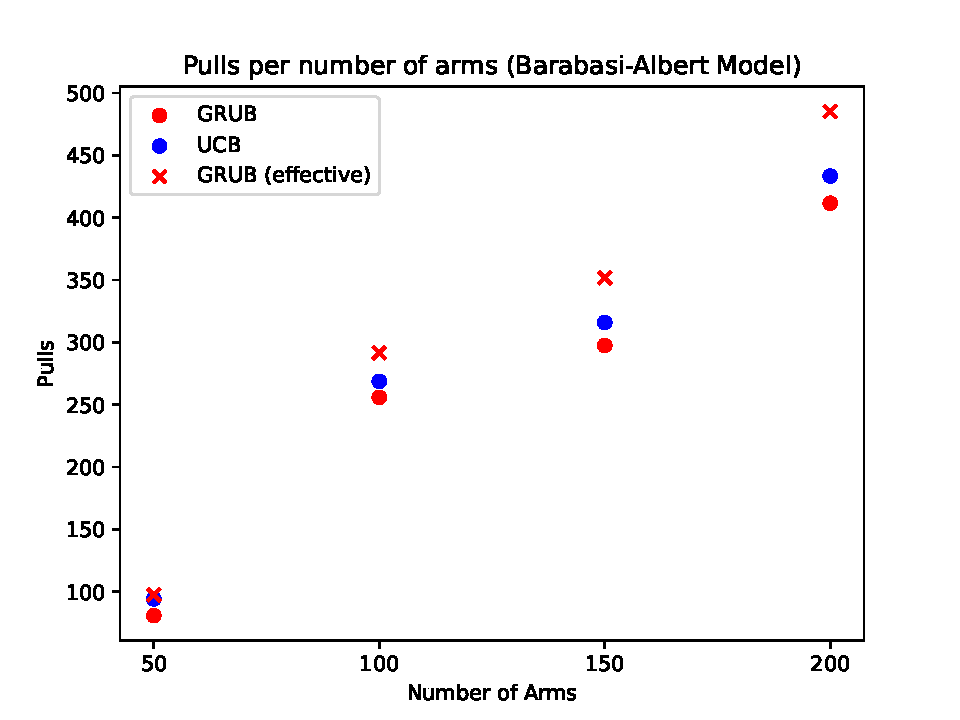
\includegraphics[width=0.45\textwidth]{../ba_figure.pdf}
    \hfill
    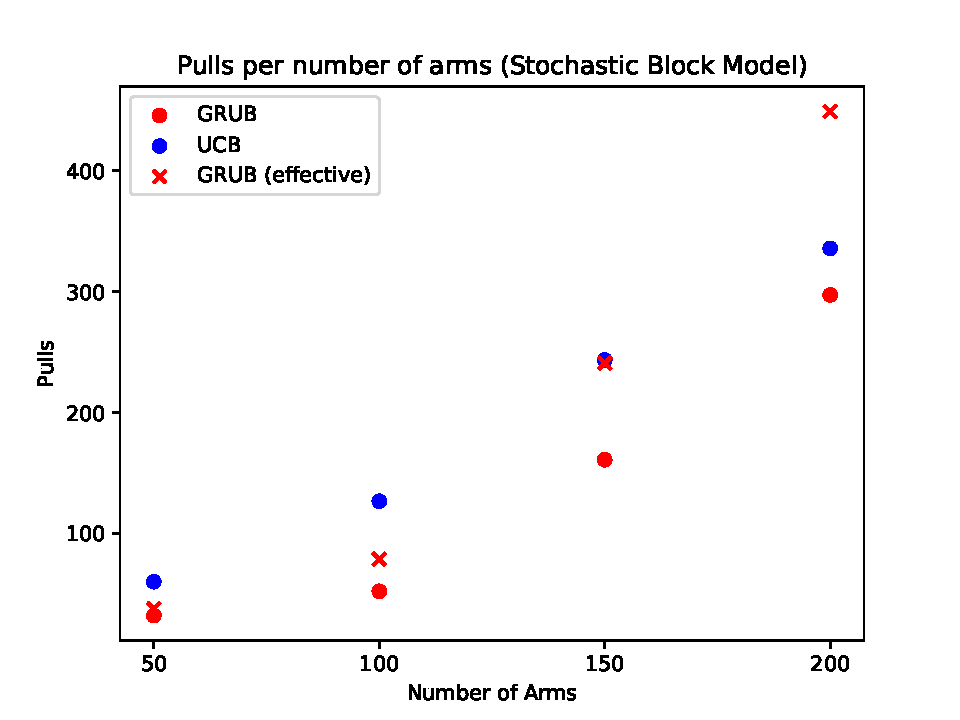
\includegraphics[width=0.45\linewidth]{../sbm_figure.pdf}
	  \caption{Results of GRUB compared with UCB on multi-armed bandits with various numbers of arms.}
    \label{fig:results}
\end{figure}

The GRUB and UCB algorithms were implemented in python and ran in an attempt to replicate a portion of the results seen in Figure 1 of the paper.
Figure \ref{fig:results} shows the results when our GRUB and UCB implementations were run on 2 synthetic datasets.
Specifically, the results shown show compare performance of GRUB and UCB on datasets generated from the Stochastic Block and Barabasi-Albert models.
Like the results of the paper, the values shown at each point are the combined results of the algorithm on 20 different model instances. \\

It is worth noting that the authors of the paper released their source code publicly.
Their implementation was not viewed or used as a reference in the construction of ours in any way.
This likely explains the differences in our results. \\

One aspect unexplained by the paper is how to generate the underlying means from the graph information.
The paper details the mechanism to quantify the smoothness of a graph given the laplacian and means,
but does not detail how to construct means from a given graph.
We implemented a covariance-based mechanism that utilizes the graph associativity information to generate the means.
This allowed us to generate synthetic data and quantify their smoothness,
but it is unknown if our set is comparable to the results of the paper. \\

Like in the paper, our results show that GRUB can outperform UCB in all cases.
In addition to the actual number of pulls taken by GRUB, the effective number of pulls is also shown.
This shows how much additional information gained by GRUB from the graph information -
GRUB frequently finds the best arm with less pulls because it learns more per pull. \\


The source code to run our implementation of these algorithms (as well as a script to generate the above figures)
is available \href{https://github.com/sstalley/RPE_GRUB}{here}. \\




\pagebreak

\section{Algorithm Modifications and Applications}

GRUB is an algorithm designed to find the best arm in terms of reward.
It solves the pure-exploration variant of the multi-armed bandit problem when graphical similarity information is available for the arms.
GRUB can solve any problem that can be re-framed into this problem of best-arm identification. \\

Unfortunately GRUB is only applicable to similarity graphs, making it’s utility limited for more general graph-based problems.
Biological sciences, particularly the field of Bioinformatics makes extensive use of graphical data.
For example, Graphs are used to describe protein strains in epigenetics, gene sequences in genomics, interactions between proteins in proteomics, and driver interactions in metabolomics.
In these cases, the edges of the graph represent things other than similarity (such as molecular connections or chemical reactions), and as such GRUB is not applicable to this data.

\subsection{N-best arms modification}

GRUB is inherently a ``one-trick pony'' in the sense that it solves a single class of problem, limiting the number of applications where it can be used.
One modification that improves the usefulness of GRUB is to increase the set size of the arms found.
While this paper only considers the case where a single best arm is identified, this algorithm can be used to find a set of any size,
and can be modified to handle cases where the final size of the best-arms set is unknown. \\

To use GRUB to find the N-best arms the following modifications must be made:
\begin{itemize}
    \item Change the stopping condition from when $|A|=1$ to when $|A|=N$
    \item When determining if an arm is in the competitive set, use the lowest bound of the N-best arms (instead of just $a_{max}$).
    Only remove an arm from the competitive set once it is outside the lowest bound out of ALL of the current N-best arms.
\end{itemize}

This method should work for any fixed number of arms, as it will produce a set of size N that we are confident contains the best arms.
This does not handle the case where the size of the final set is unknown
(ie: if we know there is a subset of high-reward arms but the size of the subset is not known a priori).
If the range of rewards is known a priori, then we can use a fixed bound (instead of a bound derived from $a_{max}$) and eliminate arms until we are confident we have the set of arms above the fixed bound.

\subsection{Parallel Sampling}

Another limitation of GRUB is that it assumes the sampling process is purely iterative and does not consider the parallel case where multiple samples could be taken in a single time step.
This is especially important for sampling problems where the limiting factor is time. \\

Fortunately GRUB can be modified in a straightforward way to handle multiple simultaneous samples and rewards.
By adding a sampling policy that can select multiple arms (ex: MVM with the N highest margin arms), and updating $x_t$ and $V_t$ once for each arm pulled,
GRUB can handle multiple simultaneous samples per iteration.
The rest of the algorithm does not need to be modified.
It’s worth noting that this modification also reduces the per-sample computational expense of GRUB,
as $V_t$ is inverted once for each set of samples instead of once for every individual sample. \\

With these two modifications we have transformed GRUB from a sequential best-arm identifier into a parallel N-best arms identifier.
GRUB went from taking one sample at a time to identify one arm into taking multiple samples at a time to identify multiple promising arms.
This greatly expands the class of problems GRUB can be applied to.

\subsection{Distance-Penalized Boundary Estimation}

A straightforward approach to applying GRUB for the distance-penalized boundary-estimation problem would be to apply GRUB to the same graph-based sampling problem that CuP solves to find the set of cut edges.
In CuP the continuous sample space is discretized into a grid of sample locations connected by edges.
The goal is to identify the set of ``cut edges'', i.e. the set of edges that cross the boundary by sampling both ends of the edge.
GRUB could be used to find the set of ``cut edges'' by eliminating all the edges that we are confident do not cross the boundary. \\

This would require the following modifications to the algorithm:
\begin{itemize}
    \item use a fixed confidence bound instead of the lower bound of $a_{max}$.
    \item change the stopping condition from $|A|=1$ to when our set is complete (ie: when we are confident nothing else is above the fixed bound)
    \item use a sampling policy that picks edges to investigate and prioritizes nearby sample locations
    \item use a similarity graph based off of edge location. Cut edges are nearby other cut edges - a cell with one cut edge is guaranteed to contain at least one more.
    Use the similarity graph to let GRUB leverage this spatial locality.
    \item Construct a reward function that rewards finding cut edges
\end{itemize}

Note that the sampling policy would have to select a set of nodes to sample in order to uncover an edge. \\

Instead of framing this problem as finding the set of cut edges (and having each node in the similarity graph represent an edge),
one could also frame this problem as finding the set of informative sample locations (having each node in the similarity graph represent a sample location), providing a reward for each useful sample.
Informative samples are near one another, just like cut edges, so the similarity graph could still be used to leverage the spatial locality.
It is unclear which method would be superior without further investigation.

\subsection{Plant Breeding}

Traditional plant breeding programs are another such example problem.
In such programs, plants are selected, crossed, and grown for experimental purposes.
Typically the goal of such programs is to produce improved varieties of plants (ex: higher yields, unique flavors, more disease resistant, drought tolerant, etc.).
New varieties are created by selecting and cross breeding existing varieties. In this sense plant breeding is naturally a sampling problem. \\

Plants are often seasonal and take time to grow and mature, making a purely sequential selection process impractical.
Additionally, agriculture is a field that is very scalable, and while growing a plant individually can be quite expensive,
the cost per plant drops dramatically when growing multiple plants simultaneously.
For these reasons a parallel selection process is necessary. \\

Genetic diversity is another important element of plant breeding.
Breeders cannot create unique new varieties without a wide variety of genes to cross.
Monocultures, while common in commercial agriculture, are undesirable for breeding.
For that reason the goal of breeding programs is not to produce a single new variety but rather multiple new varieties.
As such, an algorithm that seeks to find multiple different ``best'' varieties with the same features is much more suited to this application. \\

With the modifications above, GRUB could be applied to a plant breeding program by having it select plants to grow over several growing seasons.
Assume we have a set of plant varieties that we want to grow to find the ``best'' varieties.
Also assume we have some similarity information about the varieties.
This information could be derived from genetic sequencing, phenotypic properties, or any other correlatable feature.
GRUB could be used to confidently find a set of the N best plants.
First we define a reward function to rate the plants, then for each season have GRUB select M plants to grow that season.
After several seasons of growing and rating the varieties, GRUB would begin to eliminate varieties that it is confident are not the best,
eventually determining the best N varieties in terms of our reward. \\

This application is motivated by regional agricultural research.
There are multiple plant breeding programs throughout the state and metro area.
Oregon State University is home to \href{https://plantbreeding.oregonstate.edu/}{nine active breeding programs},
and there are several private commercial breeding programs across the state investigating everything from Broccoli to Cannabis.

\end{document}
